% SBA MODA Workshop — Pokémon Type Classifier
% Beamer Presentation
\documentclass[aspectratio=169, 11pt]{beamer}

% Theme and colours
\usetheme{default}
\usecolortheme{beaver}
\setbeamertemplate{navigation symbols}{}
\definecolor{ausred}{RGB}{153, 0, 0}
\definecolor{firered}{RGB}{255, 107, 53}
\definecolor{waterblue}{RGB}{58, 134, 255}
\definecolor{grassgreen}{RGB}{45, 198, 83}
\setbeamercolor{title}{fg=ausred}
\setbeamercolor{frametitle}{fg=ausred}
\setbeamercolor{structure}{fg=ausred}
\setbeamertemplate{footline}[frame number]

% Packages
\usepackage{amsmath, amssymb}
\usepackage{graphicx}
\usepackage{booktabs}
\usepackage{tikz}
\usetikzlibrary{shapes, arrows, positioning, fit, backgrounds}
\usepackage{listings}
\usepackage{xcolor}
\usepackage{hyperref}

% Code style
\lstset{
    language=Python,
    basicstyle=\ttfamily\scriptsize,
    keywordstyle=\color{blue}\bfseries,
    stringstyle=\color{red!70!black},
    commentstyle=\color{green!50!black}\itshape,
    showstringspaces=false,
    breaklines=true,
    frame=single,
    backgroundcolor=\color{gray!10},
    numbers=left,
    numberstyle=\tiny\color{gray}
}

% Title information
\title[Pokémon Classifier]{Can a Machine Tell Pokémon Types Apart?}
\subtitle{SBA MODA Workshop — A Gentle Introduction to Machine Learning}
\author{Dr.\ Harshvardhan}
\institute{School of Business Administration\\American University of Sharjah}
\date{Spring 2026}

\begin{document}

% ---------- Title ----------
\begin{frame}
    \titlepage
    \begin{tikzpicture}[remember picture, overlay]
        \node[anchor=south east, xshift=-0.5cm, yshift=0.5cm] at (current page.south east) {
            
\includegraphics[height=1.5cm]{aus.png}
        };
    \end{tikzpicture}
\end{frame}

% ---------- Welcome ----------
\begin{frame}{Welcome!}
    Today we will build, together, a small piece of machine learning.

    \vspace{0.4cm}
    \begin{itemize}
        \item No prior coding experience required
        \item No prior machine-learning experience required
        \item Bring curiosity, a laptop, and a browser
    \end{itemize}

    \vspace{0.4cm}
    \textbf{Our goal:} teach a computer to look at a Pokémon and guess whether it is \textcolor{firered}{Fire}, \textcolor{waterblue}{Water}, or \textcolor{grassgreen}{Grass}.

    \vspace{0.4cm}
    \begin{center}
    
\includegraphics[height=2.5cm]{figures/charmander.png}\hspace{0.5cm}
    
\includegraphics[height=2.5cm]{figures/squirtle.png}\hspace{0.5cm}
    
\includegraphics[height=2.5cm]{figures/bulbasaur.png}
    \end{center}
\end{frame}

% ===================================================================
\section{Part 1: What is Machine Learning?}
% ===================================================================
\begin{frame}
    \centering
    \Huge \textcolor{ausred}{Part 1}

    \vspace{0.5cm}
    \LARGE What \emph{is} Machine Learning?
\end{frame}

% ---------- AI is everywhere ----------
\begin{frame}{Artificial Intelligence is already in your pocket}
    AI = computers doing things that look intelligent.

    \vspace{0.4cm}
    \begin{columns}[T]
        \column{0.5\textwidth}
        \textbf{Examples you use every day:}
        \begin{itemize}
            \item Gmail filtering spam
            \item Netflix recommending shows
            \item Face unlock on your phone
            \item Google Translate
            \item ChatGPT
        \end{itemize}

        \column{0.5\textwidth}
        \textbf{Examples in business:}
        \begin{itemize}
            \item Bank fraud detection
            \item Credit-score prediction
            \item Demand forecasting
            \item Chatbots in customer service
            \item Pricing optimisation
        \end{itemize}
    \end{columns}
\end{frame}

% ---------- ML inside AI ----------
\begin{frame}{Machine Learning is how modern AI learns}
    \begin{columns}[T]
        \column{0.5\textwidth}
        \textbf{The old way: programming}

        \vspace{0.2cm}
        Write rules by hand:
        \vspace{0.2cm}

        \texttt{IF email has ``free money''} \\
        \texttt{AND lots of !!!} \\
        \texttt{THEN it is spam}

        \vspace{0.4cm}
        \textcolor{red}{Brittle. Spammers change tricks. New rules needed every week.}

        \column{0.5\textwidth}
        \textbf{The new way: machine learning}

        \vspace{0.2cm}
        Show the computer 100{,}000 emails labelled \emph{spam} / \emph{not spam}.

        \vspace{0.4cm}
        It \emph{learns} the pattern itself.

        \vspace{0.4cm}
        \textcolor{green!50!black}{Adapts as spammers evolve.}
    \end{columns}
\end{frame}

% ---------- Data ----------
\begin{frame}{What is ``data'' anyway?}
    \begin{columns}[T]
        \column{0.55\textwidth}
        Data is just \textbf{numbers organised in a table}.

        \vspace{0.3cm}

        \begin{tabular}{lccc}
        \toprule
        Pokémon & Avg R & Avg G & Avg B \\
        \midrule
        Charmander & 240 & 200 & 150 \\
        Squirtle   & 180 & 210 & 240 \\
        Bulbasaur  & 200 & 230 & 180 \\
        \bottomrule
        \end{tabular}

        \vspace{0.4cm}

        Each \textbf{row} is one example.\\
        Each \textbf{column} is one feature.

        \column{0.45\textwidth}
        \centering
        
\includegraphics[height=2cm]{figures/charmander.png}\\
        
\includegraphics[height=2cm]{figures/squirtle.png}\\
        
\includegraphics[height=2cm]{figures/bulbasaur.png}
    \end{columns}
\end{frame}

% ---------- Supervised learning ----------
\begin{frame}{Supervised learning, in one picture}
    \centering
    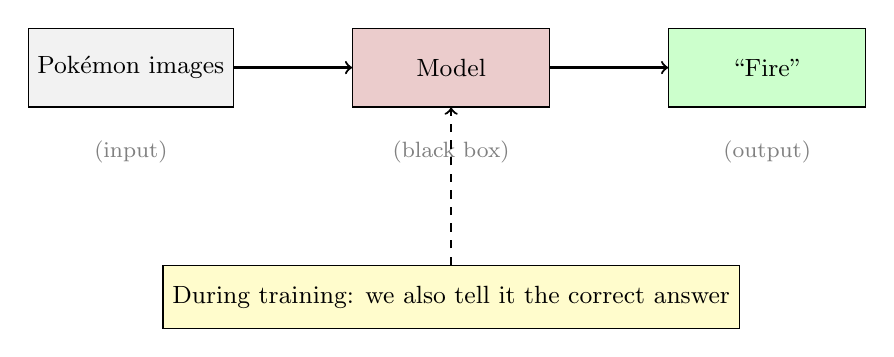
\begin{tikzpicture}[node distance=1.5cm, font=\small]
        \node[draw, rectangle, fill=gray!10, minimum width=2.5cm, minimum height=1cm] (data) {Pokémon images};
        \node[draw, rectangle, fill=ausred!20, right=of data, minimum width=2.5cm, minimum height=1cm] (model) {Model};
        \node[draw, rectangle, fill=green!20, right=of model, minimum width=2.5cm, minimum height=1cm] (pred) {``Fire''};
        \node[below=0.3cm of data, font=\footnotesize, gray] {(input)};
        \node[below=0.3cm of model, font=\footnotesize, gray] {(black box)};
        \node[below=0.3cm of pred, font=\footnotesize, gray] {(output)};
        \draw[->, thick] (data) -- (model);
        \draw[->, thick] (model) -- (pred);

        \node[draw, rectangle, fill=yellow!20, below=2cm of model, minimum width=4cm, minimum height=0.8cm] (label) {During training: we also tell it the correct answer};
        \draw[->, thick, dashed] (label.north) -- (model.south);
    \end{tikzpicture}

    \vspace{0.5cm}
    The model adjusts itself to match the labels we provide.
\end{frame}

% ---------- Train / test ----------
\begin{frame}{The most important idea: train vs.\ test}
    \begin{columns}[T]
        \column{0.55\textwidth}
        \textbf{Analogy: studying for an exam.}

        \vspace{0.3cm}
        You study from a textbook (the \emph{training set}).

        \vspace{0.3cm}
        Then you take the exam, where the questions are \emph{new} (the \emph{test set}).

        \vspace{0.3cm}
        If we let the model peek at the exam, of course it gets 100\%. That tells us nothing.

        \vspace{0.4cm}
        \textcolor{ausred}{\textbf{Always hold out unseen data for the final test.}}

        \column{0.45\textwidth}
        \centering
        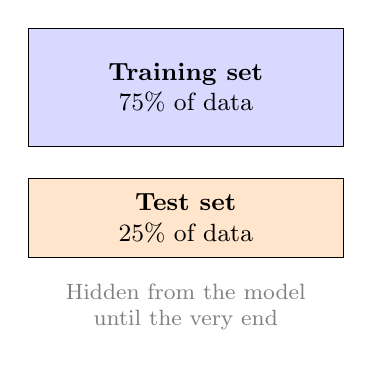
\begin{tikzpicture}[font=\small]
            \node[draw, rectangle, fill=blue!15, minimum width=4cm, minimum height=1.5cm, align=center] (train) {\textbf{Training set}\\75\% of data};
            \node[draw, rectangle, fill=orange!20, below=0.4cm of train, minimum width=4cm, minimum height=1cm, align=center] (test) {\textbf{Test set}\\25\% of data};
            \node[below=0.2cm of test, font=\footnotesize, gray, align=center] {Hidden from the model\\until the very end};
        \end{tikzpicture}
    \end{columns}
\end{frame}

% ===================================================================
\section{Part 2: How a Computer Sees an Image}
% ===================================================================
\begin{frame}
    \centering
    \Huge \textcolor{ausred}{Part 2}

    \vspace{0.5cm}
    \LARGE How a Computer Sees an Image
\end{frame}

% ---------- Image is numbers ----------
\begin{frame}{Pictures are secretly grids of numbers}
    \centering
    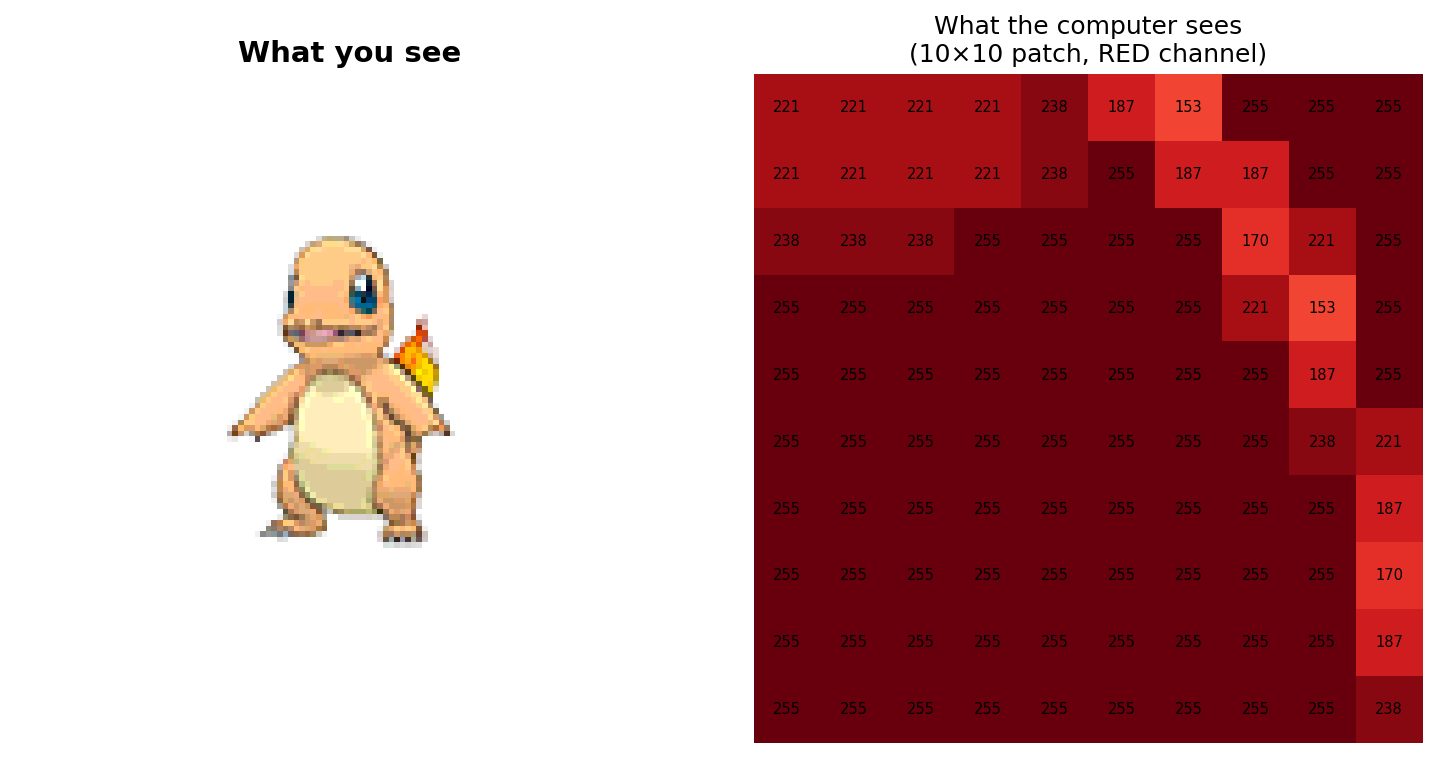
\includegraphics[width=0.92\textwidth]{figures/image_vs_numbers.png}

    \vspace{0.3cm}
    Each pixel is a brightness value from 0 (black) to 255 (full colour).
\end{frame}

% ---------- RGB ----------
\begin{frame}{Three colour channels: Red, Green, Blue}
    \centering
    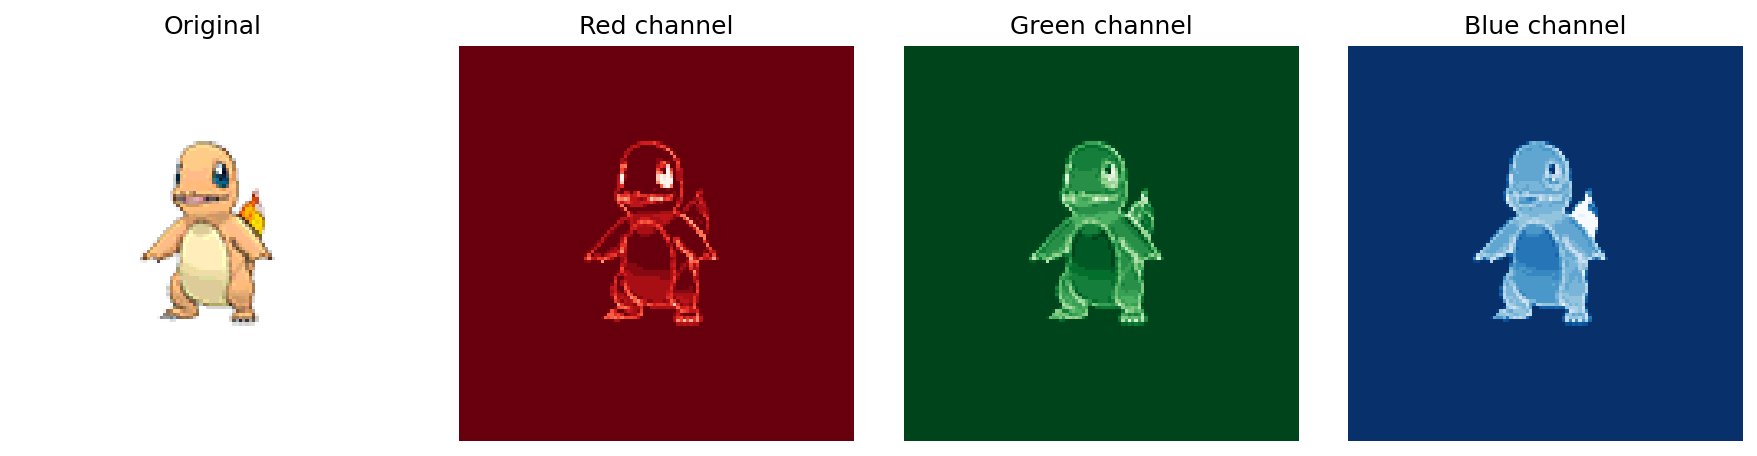
\includegraphics[width=0.95\textwidth]{figures/rgb_channels.png}

    \vspace{0.4cm}
    Stack the three together $\rightarrow$ full-colour image.
\end{frame}

% ---------- Image is BIG ----------
\begin{frame}{One image = a LOT of numbers}
    \centering
    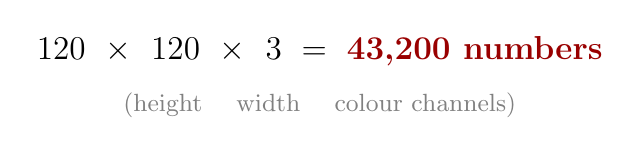
\begin{tikzpicture}[font=\large]
        \node {120 \;$\times$\; 120 \;$\times$\; 3 \;=\; \textcolor{ausred}{\textbf{43{,}200 numbers}}};
        \node[below=0.4cm, font=\small, gray] {(height \quad width \quad colour channels)};
    \end{tikzpicture}

    \vspace{0.6cm}
    That's a lot of numbers per Pokémon.

    \vspace{0.3cm}
    A simple model with so many inputs would either:
    \begin{itemize}
        \item train painfully slowly, or
        \item just memorise the training images and fail on new ones.
    \end{itemize}

    \vspace{0.4cm}
    \textcolor{ausred}{\textbf{We need to summarise.}}
\end{frame}

% ===================================================================
\section{Part 3: Features}
% ===================================================================
\begin{frame}
    \centering
    \Huge \textcolor{ausred}{Part 3}

    \vspace{0.5cm}
    \LARGE Features: turning images into a few numbers
\end{frame}

% ---------- Features ----------
\begin{frame}{A feature is a summary number}
    \textbf{Idea:} replace the 43{,}200 pixel values by a small list of \emph{descriptive} numbers.

    \vspace{0.4cm}
    For Pokémon, the simplest meaningful summary is the \textbf{average} amount of red, green, and blue across all pixels.

    \vspace{0.5cm}
    \centering
    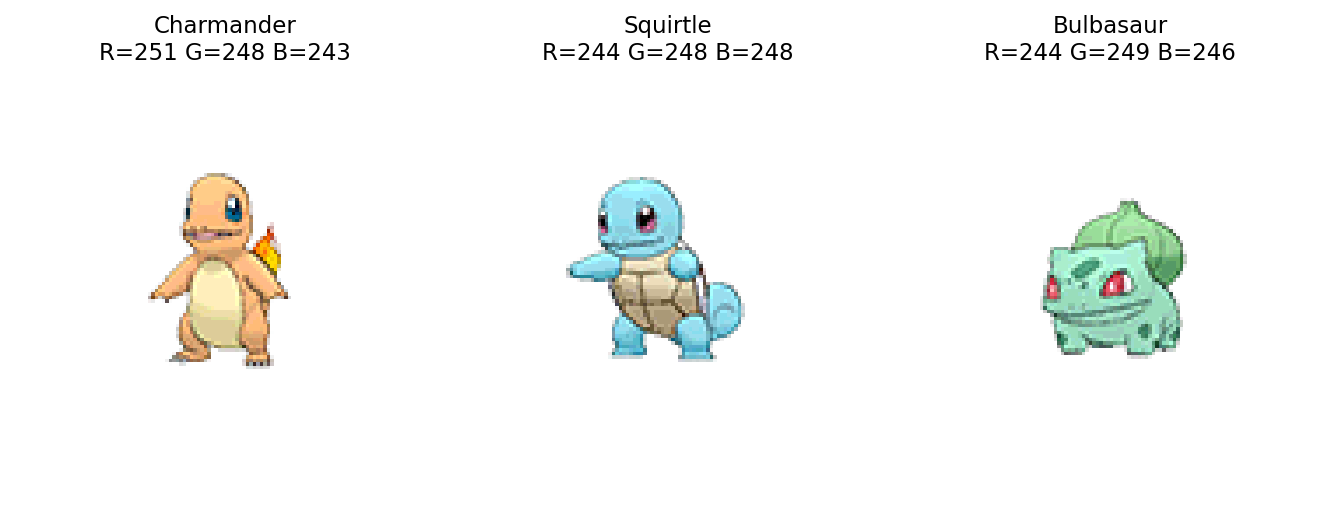
\includegraphics[width=0.95\textwidth]{figures/average_colors.png}
\end{frame}

% ---------- Feature scatter ----------
\begin{frame}{Why this works for Pokémon}
    \centering
    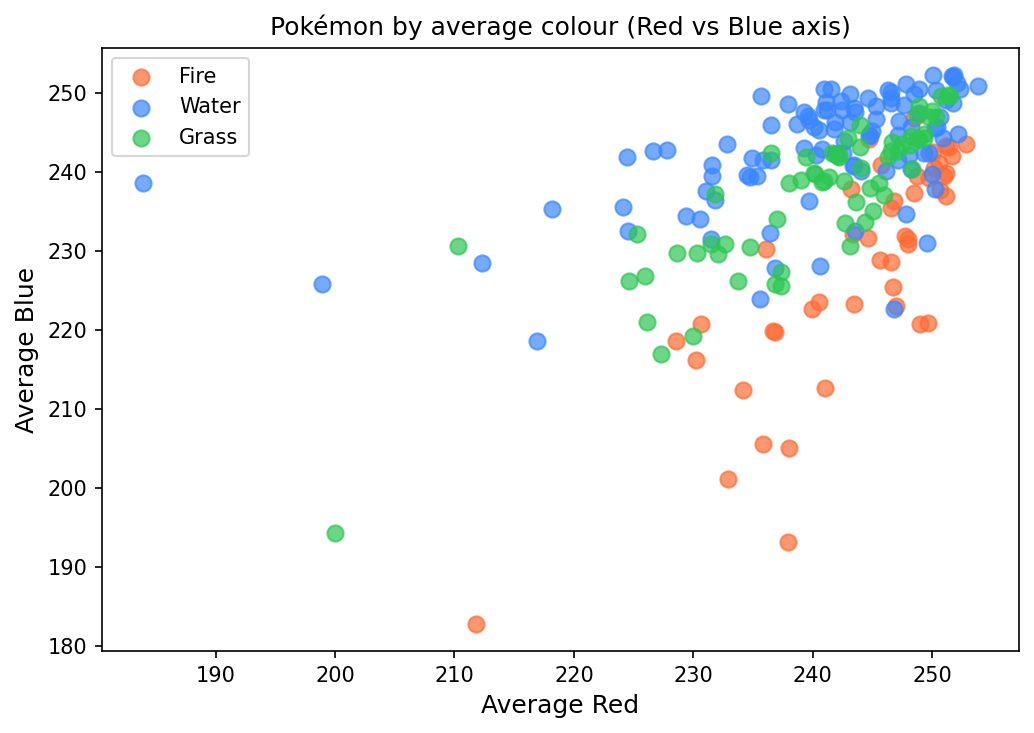
\includegraphics[width=0.7\textwidth]{figures/pokemon_scatter.png}

    \vspace{0.3cm}
    Just two of the three colour averages already separate the types nicely.
\end{frame}

% ---------- Pipeline ----------
\begin{frame}{The complete pipeline}
    \centering
    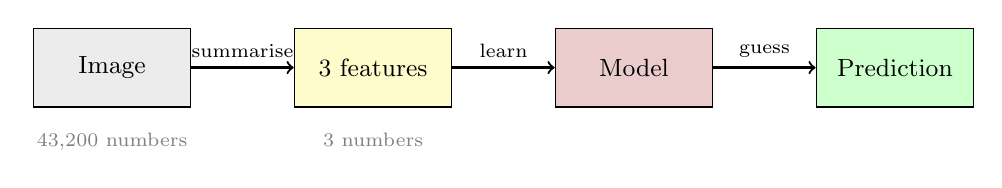
\begin{tikzpicture}[node distance=1.3cm, font=\small]
        \node[draw, rectangle, fill=gray!15, minimum width=2cm, minimum height=1cm] (img) {Image};
        \node[draw, rectangle, fill=yellow!20, right=of img, minimum width=2cm, minimum height=1cm] (feat) {3 features};
        \node[draw, rectangle, fill=ausred!20, right=of feat, minimum width=2cm, minimum height=1cm] (model) {Model};
        \node[draw, rectangle, fill=green!20, right=of model, minimum width=2cm, minimum height=1cm] (pred) {Prediction};

        \draw[->, thick] (img) -- node[above, font=\scriptsize]{summarise} (feat);
        \draw[->, thick] (feat) -- node[above, font=\scriptsize]{learn} (model);
        \draw[->, thick] (model) -- node[above, font=\scriptsize]{guess} (pred);

        \node[below=0.2cm of img, font=\scriptsize, gray] {43{,}200 numbers};
        \node[below=0.2cm of feat, font=\scriptsize, gray] {3 numbers};
    \end{tikzpicture}

    \vspace{0.5cm}
    \textbf{Feature engineering} is the art of choosing those summary numbers wisely.
\end{frame}

% ===================================================================
\section{Part 4: Two Kinds of Models}
% ===================================================================
\begin{frame}
    \centering
    \Huge \textcolor{ausred}{Part 4}

    \vspace{0.5cm}
    \LARGE Two kinds of models we will try
\end{frame}

% ---------- Decision tree ----------
\begin{frame}{Decision tree: a flowchart of yes/no questions}
    \centering
    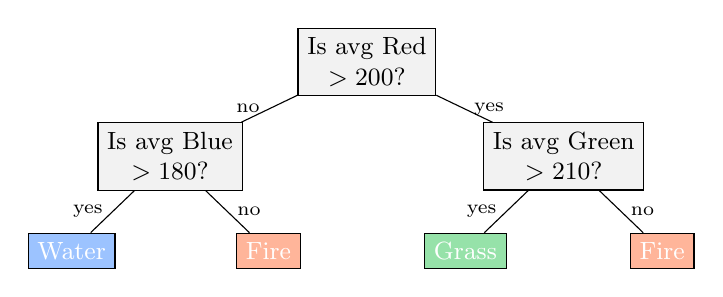
\begin{tikzpicture}[
        level distance=1.2cm,
        level 1/.style={sibling distance=5cm},
        level 2/.style={sibling distance=2.5cm},
        every node/.style={font=\small},
        node/.style={draw, rectangle, fill=gray!10, minimum width=1.6cm, align=center}
    ]
        \node[draw, rectangle, fill=gray!10, align=center] {Is avg Red\\$> 200$?}
            child {
                node[draw, rectangle, fill=gray!10, align=center] {Is avg Blue\\$> 180$?}
                    child { node[draw, rectangle, fill=waterblue!50, text=white]{Water} edge from parent node[left, font=\scriptsize]{yes}}
                    child { node[draw, rectangle, fill=firered!50, text=white]{Fire} edge from parent node[right, font=\scriptsize]{no}}
                edge from parent node[left, font=\scriptsize]{no}
            }
            child {
                node[draw, rectangle, fill=gray!10, align=center] {Is avg Green\\$> 210$?}
                    child { node[draw, rectangle, fill=grassgreen!50, text=white]{Grass} edge from parent node[left, font=\scriptsize]{yes}}
                    child { node[draw, rectangle, fill=firered!50, text=white]{Fire} edge from parent node[right, font=\scriptsize]{no}}
                edge from parent node[right, font=\scriptsize]{yes}
            };
    \end{tikzpicture}

    \vspace{0.3cm}
    The computer figures out the questions and the thresholds itself.
\end{frame}

% ---------- Random forest ----------
\begin{frame}{Random Forest: many trees voting}
    \centering
    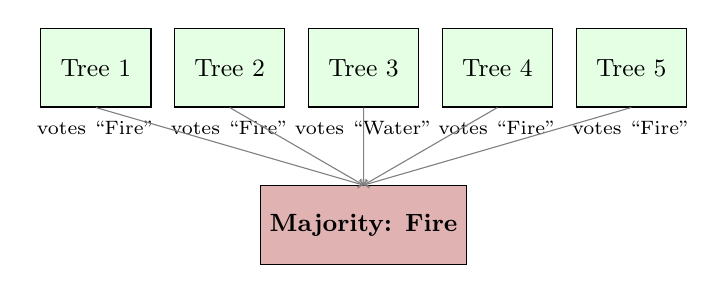
\begin{tikzpicture}[font=\small]
        \foreach \i/\v in {1/Fire, 2/Fire, 3/Water, 4/Fire, 5/Fire} {
            \node[draw, rectangle, fill=green!10, minimum width=1.4cm, minimum height=1cm]
                at (\i*1.7, 2) (t\i) {Tree \i};
            \node[font=\scriptsize, below=0.05cm of t\i] {votes ``\v''};
        }
        \node[draw, rectangle, fill=ausred!30, minimum width=2.5cm, minimum height=1cm] (out) at (5.1, 0) {\textbf{Majority: Fire}};
        \foreach \i in {1, 2, 3, 4, 5} {
            \draw[->, gray] (t\i.south) -- (out.north);
        }
    \end{tikzpicture}

    \vspace{0.4cm}
    \begin{itemize}
        \item Build many decision trees, each on a different slice of the data
        \item Each tree votes on a new Pokémon
        \item The majority answer wins
        \item Almost always more accurate than a single tree
    \end{itemize}
\end{frame}

% ---------- Logistic regression ----------
\begin{frame}{Logistic Regression: draw straight lines between classes}
    \begin{columns}[T]
        \column{0.5\textwidth}
        Imagine plotting every Pokémon as a dot in feature space (e.g.\ Red on x-axis, Blue on y-axis).

        \vspace{0.4cm}
        Logistic Regression \emph{draws straight lines} that separate the classes.

        \vspace{0.4cm}
        Despite the name, it does \textbf{classification}, not regression.

        \column{0.5\textwidth}
        \centering
        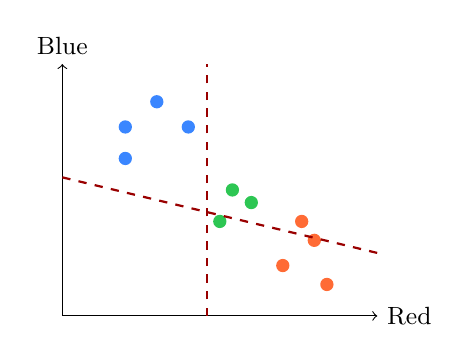
\begin{tikzpicture}[scale=0.8]
            \draw[->] (0,0) -- (5,0) node[right, font=\small] {Red};
            \draw[->] (0,0) -- (0,4) node[above, font=\small] {Blue};
            \fill[firered] (3.5, 0.8) circle (3pt);
            \fill[firered] (4, 1.2) circle (3pt);
            \fill[firered] (4.2, 0.5) circle (3pt);
            \fill[firered] (3.8, 1.5) circle (3pt);
            \fill[waterblue] (1, 3) circle (3pt);
            \fill[waterblue] (1.5, 3.4) circle (3pt);
            \fill[waterblue] (2, 3) circle (3pt);
            \fill[waterblue] (1, 2.5) circle (3pt);
            \fill[grassgreen] (2.5, 1.5) circle (3pt);
            \fill[grassgreen] (2.7, 2) circle (3pt);
            \fill[grassgreen] (3, 1.8) circle (3pt);
            \draw[ausred, thick, dashed] (0, 2.2) -- (5, 1);
            \draw[ausred, thick, dashed] (2.3, 0) -- (2.3, 4);
        \end{tikzpicture}
    \end{columns}
\end{frame}

% ---------- Two models compared ----------
\begin{frame}{Trees versus lines}
    \begin{columns}[T]
        \column{0.5\textwidth}
        \textbf{Random Forest}
        \begin{itemize}
            \item Many flexible trees
            \item Captures complex non-linear patterns
            \item Needs more data + features
            \item Harder to interpret
        \end{itemize}

        \column{0.5\textwidth}
        \textbf{Logistic Regression}
        \begin{itemize}
            \item Single straight-line model
            \item Best when classes \emph{are} roughly linearly separable
            \item Fast and simple
            \item Easy to explain
        \end{itemize}
    \end{columns}

    \vspace{0.6cm}
    \begin{center}
    \textcolor{ausred}{\textbf{Which one wins for Pokémon? Let's find out in the notebook.}}
    \end{center}
\end{frame}

% ===================================================================
\section{Part 5: How do we know if it worked?}
% ===================================================================
\begin{frame}
    \centering
    \Huge \textcolor{ausred}{Part 5}

    \vspace{0.5cm}
    \LARGE How do we know if it worked?
\end{frame}

% ---------- Accuracy ----------
\begin{frame}{Accuracy: the simplest score}
    \begin{center}
        \Large
        Accuracy $=$ \textcolor{ausred}{\textbf{number correct}} / total
    \end{center}

    \vspace{0.5cm}
    Out of 55 test Pokémon:
    \begin{itemize}
        \item 42 right $\rightarrow$ \textbf{76\% accuracy}
        \item 30 right $\rightarrow$ \textbf{55\% accuracy}
    \end{itemize}

    \vspace{0.4cm}
    Easy to compute. Easy to explain.
\end{frame}

% ---------- CM intro ----------
\begin{frame}{Accuracy hides where the model failed}
    A model with 76\% accuracy got 24\% wrong. \textbf{Where} did the mistakes come from?

    \vspace{0.4cm}
    \begin{itemize}
        \item Did it confuse Fire with Water? (the colours are far apart)
        \item Did it confuse Grass with Water? (some plants are blue-ish)
        \item Did it always predict ``Water'' because that's the most common type?
    \end{itemize}

    \vspace{0.4cm}
    A single number can't tell us. We need a \textbf{confusion matrix}.
\end{frame}

% ---------- Confusion matrix ----------
\begin{frame}{Confusion matrix}
    \begin{columns}[T]
        \column{0.5\textwidth}
        \centering
        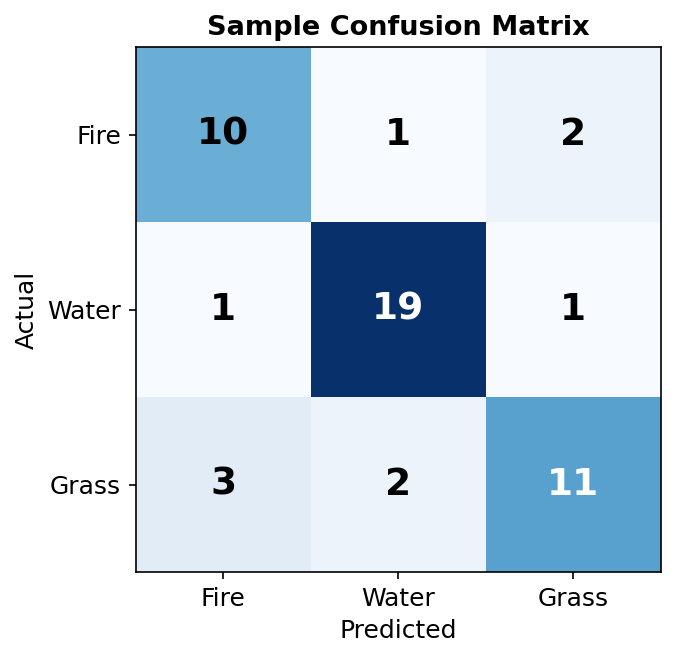
\includegraphics[width=\textwidth]{figures/confusion_matrix_example.png}

        \column{0.5\textwidth}
        \begin{itemize}
            \item \textbf{Diagonal} = correct predictions
            \item \textbf{Off-diagonal} = mistakes
            \item \textbf{Rows} = the actual type
            \item \textbf{Columns} = what the model predicted
        \end{itemize}

        \vspace{0.4cm}

        Lets us see exactly which classes the model gets confused between.
    \end{columns}
\end{frame}

% ===================================================================
\section{Part 6: Tuning the model}
% ===================================================================
\begin{frame}
    \centering
    \Huge \textcolor{ausred}{Part 6}

    \vspace{0.5cm}
    \LARGE Tuning the model
\end{frame}

% ---------- Hyperparameters ----------
\begin{frame}{Models have knobs: hyperparameters}
    \begin{columns}[T]
        \column{0.6\textwidth}
        \textbf{Random Forest knobs:}
        \begin{itemize}
            \item \texttt{n\_estimators} — how many trees?
            \item \texttt{max\_depth} — how deep can a tree grow?
            \item \texttt{min\_samples\_leaf} — how few examples in a leaf?
        \end{itemize}

        \vspace{0.3cm}
        \textbf{Logistic Regression knobs:}
        \begin{itemize}
            \item \texttt{C} — how strongly to penalise complex boundaries?
            \item \texttt{max\_iter} — how long to keep optimising?
        \end{itemize}

        \column{0.4\textwidth}
        \centering
        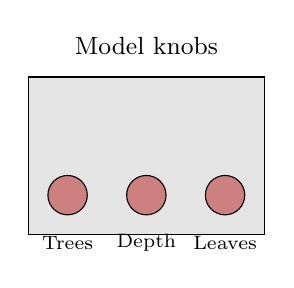
\begin{tikzpicture}
            \draw[fill=gray!20] (0,0) rectangle (3, 2);
            \node at (1.5, 2.4) {\small Model knobs};
            \foreach \i/\name in {0.5/Trees, 1.5/Depth, 2.5/Leaves} {
                \draw[fill=ausred!50] (\i, 0.5) circle (0.25);
                \node[font=\scriptsize] at (\i, -0.1) {\name};
            }
        \end{tikzpicture}

        \vspace{0.5cm}
        Different settings $\rightarrow$ different performance.
    \end{columns}
\end{frame}

% ---------- CV ----------
\begin{frame}{Cross-validation: a fairer test during training}
    Split the training data into 5 chunks. For each setting:
    \begin{enumerate}
        \item Train on 4 chunks, test on 1
        \item Repeat 5 times, rotating which chunk is held out
        \item Average the 5 scores
    \end{enumerate}

    \vspace{0.3cm}
    \centering
    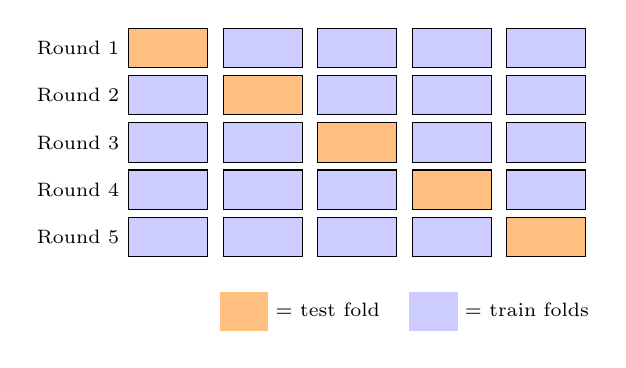
\begin{tikzpicture}[font=\small]
        \foreach \r in {1, 2, 3, 4, 5} {
            \foreach \c in {1, 2, 3, 4, 5} {
                \pgfmathtruncatemacro{\test}{\r==\c ? 1 : 0}
                \ifnum\test=1
                    \fill[orange!50] (\c*1.2, -\r*0.6) rectangle ++(1, 0.5);
                \else
                    \fill[blue!20] (\c*1.2, -\r*0.6) rectangle ++(1, 0.5);
                \fi
                \draw (\c*1.2, -\r*0.6) rectangle ++(1, 0.5);
            }
            \node[left] at (1.2, -\r*0.6+0.25) {\scriptsize Round \r};
        }
        \node[font=\scriptsize] at (4.7, -3.7) {\colorbox{orange!50}{\strut\hspace{0.4cm}} = test fold \quad \colorbox{blue!20}{\strut\hspace{0.4cm}} = train folds};
    \end{tikzpicture}
\end{frame}

% ---------- GridSearch ----------
\begin{frame}{GridSearchCV: try every combination automatically}
    \begin{columns}[T]
        \column{0.55\textwidth}
        We give the computer a \textbf{grid} of values:
        \vspace{0.2cm}

        \begin{tabular}{ll}
        \texttt{n\_estimators} & 50, 100, 200 \\
        \texttt{max\_depth}    & 3, 5, 10 \\
        \end{tabular}

        \vspace{0.3cm}
        That's $3 \times 3 = 9$ combinations.

        \vspace{0.3cm}
        For each one, it runs 5-fold cross-validation:\\
        $9 \times 5 = 45$ small experiments.

        \vspace{0.3cm}
        It returns the best-scoring combination.

        \column{0.45\textwidth}
        \centering
        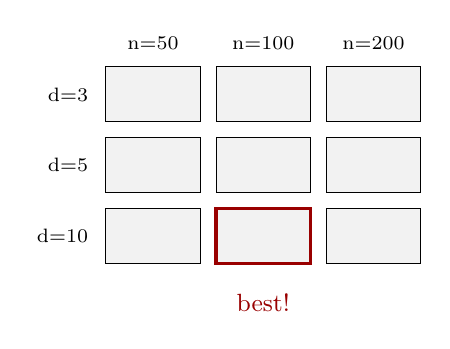
\begin{tikzpicture}[font=\scriptsize]
            % Grid cells
            \foreach \r in {0, 1, 2} {
                \foreach \c in {0, 1, 2} {
                    \draw[fill=gray!10] (0.4 + \c*1.4, -0.4 - \r*0.9) rectangle ++(1.2, 0.7);
                }
            }
            % Column headers (n_estimators)
            \node at (1.0, 0.6) {n=50};
            \node at (2.4, 0.6) {n=100};
            \node at (3.8, 0.6) {n=200};
            % Row headers (max_depth)
            \node[anchor=east] at (0.3, -0.05) {d=3};
            \node[anchor=east] at (0.3, -0.95) {d=5};
            \node[anchor=east] at (0.3, -1.85) {d=10};
            % Highlight best (n=100, d=10)
            \draw[ausred, very thick] (1.8, -2.2) rectangle (3.0, -1.5);
            \node[ausred, font=\small] at (2.4, -2.7) {best!};
        \end{tikzpicture}
    \end{columns}
\end{frame}

% ===================================================================
\section{Part 7: The Two Big Lessons}
% ===================================================================
\begin{frame}
    \centering
    \Huge \textcolor{ausred}{Part 7}

    \vspace{0.5cm}
    \LARGE Two big lessons before we open the notebook
\end{frame}

% ---------- Lesson 1 ----------
\begin{frame}{Lesson 1 — Tuning is useful but not magic}
    \vspace{0.5cm}
    \begin{center}
        \Large
        Hyperparameter tuning often gives you a small bump.

        \vspace{0.5cm}
        Sometimes it gives you nothing at all.

        \vspace{0.5cm}
        Occasionally it makes things worse.
    \end{center}

    \vspace{0.6cm}
    Don't expect tuning to rescue a poorly-chosen model.
\end{frame}

% ---------- Lesson 2 ----------
\begin{frame}{Lesson 2 — Picking the right model often matters more}
    \vspace{0.5cm}
    \begin{center}
        \Large
        A simple model that fits the problem\\
        beats a complex model that doesn't.

        \vspace{0.5cm}
        \textcolor{waterblue}{Logistic Regression} $>$\\\textcolor{firered}{Random Forest} for our Pokémon problem.
    \end{center}

    \vspace{0.6cm}
    Always try a simple baseline first.
\end{frame}

% ===================================================================
\section{Time to code!}
% ===================================================================
\begin{frame}
    \centering
    \Huge \textcolor{ausred}{Time to code!}

    \vspace{1cm}
    \large
    Open the notebook in Google Colab\\
    and we will run through it together.

    \vspace{1cm}
    \texttt{\small github.com/harshvardhaniimi/pokemon-workshop}
\end{frame}

% ---------- Recap ----------
\begin{frame}{What you have learned today}
    \begin{enumerate}
        \item AI \& ML are everywhere; ML learns from data instead of explicit rules
        \item Always split your data into a training set and a test set
        \item An image is just a grid of numbers (R, G, B per pixel)
        \item Features are summary numbers that describe each example
        \item Decision trees, Random Forests, and Logistic Regression are three classic model families
        \item Accuracy + confusion matrix tell you \emph{how well} and \emph{where} a model fails
        \item GridSearchCV with cross-validation tunes hyperparameters honestly
    \end{enumerate}

    \vspace{0.4cm}
    \textcolor{ausred}{\textbf{Most important takeaway:} picking the right model that fits your problem matters more than tuning a fancy one.}

    \vspace{0.3cm}
    \footnotesize\textit{Bonus material on PCA is at the end of the notebook — try it at home.}
\end{frame}

% ---------- Questions ----------
\begin{frame}
    \centering
    \Huge Questions?

    \vspace{1cm}

    \normalsize
    \texttt{harshvardhan@aus.edu}

    \vspace{0.5cm}
    School of Business Administration\\
    American University of Sharjah
\end{frame}

\end{document}
